\documentclass[12pt,letterpaper]{article}
\usepackage{fullpage}
\usepackage[top=2cm, bottom=4.5cm, left=2.5cm, right=2.5cm]{geometry}
\usepackage{amsmath,amsthm,amsfonts,amssymb,amscd}
\usepackage{lastpage}
\usepackage{enumerate}
\usepackage{fancyhdr}
\usepackage{mathrsfs}
\usepackage{xcolor}
\usepackage{graphicx}
\usepackage{listings}
\usepackage{hyperref}

\hypersetup{%
  colorlinks=true,
  linkcolor=blue,
  linkbordercolor={0 0 1}
}
 
\renewcommand\lstlistingname{Algorithm}
\renewcommand\lstlistlistingname{Algorithms}
\def\lstlistingautorefname{Alg.}

\lstdefinestyle{Python}{
    language        = Python,
    frame           = lines, 
    basicstyle      = \footnotesize,
    keywordstyle    = \color{blue},
    stringstyle     = \color{green},
    commentstyle    = \color{red}\ttfamily
}

\setlength{\parindent}{0.0in}
\setlength{\parskip}{0.05in}

% Edit these as appropriate
\newcommand\course{Computaitonal Physics}
\newcommand\hwnumber{3}                  % <-- homework number
\newcommand\NetIDa{Jiachen Wan N19996964}           % <-- NetID of person #1


\pagestyle{fancyplain}
\headheight 35pt
\lhead{\NetIDa}
\lhead{\NetIDa\\\NetIDb}                 % <-- Comment this line out for problem sets (make sure you are person #1)
\chead{\textbf{\Large Homework \hwnumber}}
\rhead{\course \\ \today}
\lfoot{}
\cfoot{}
\rfoot{\small\thepage}
\headsep 1.5em

\begin{document}

\section*{Problem 1}

\begin{enumerate}
  \item
   To start with, the sunspot plot looks like:
   
   \begin{figure}[h]
    \centering
    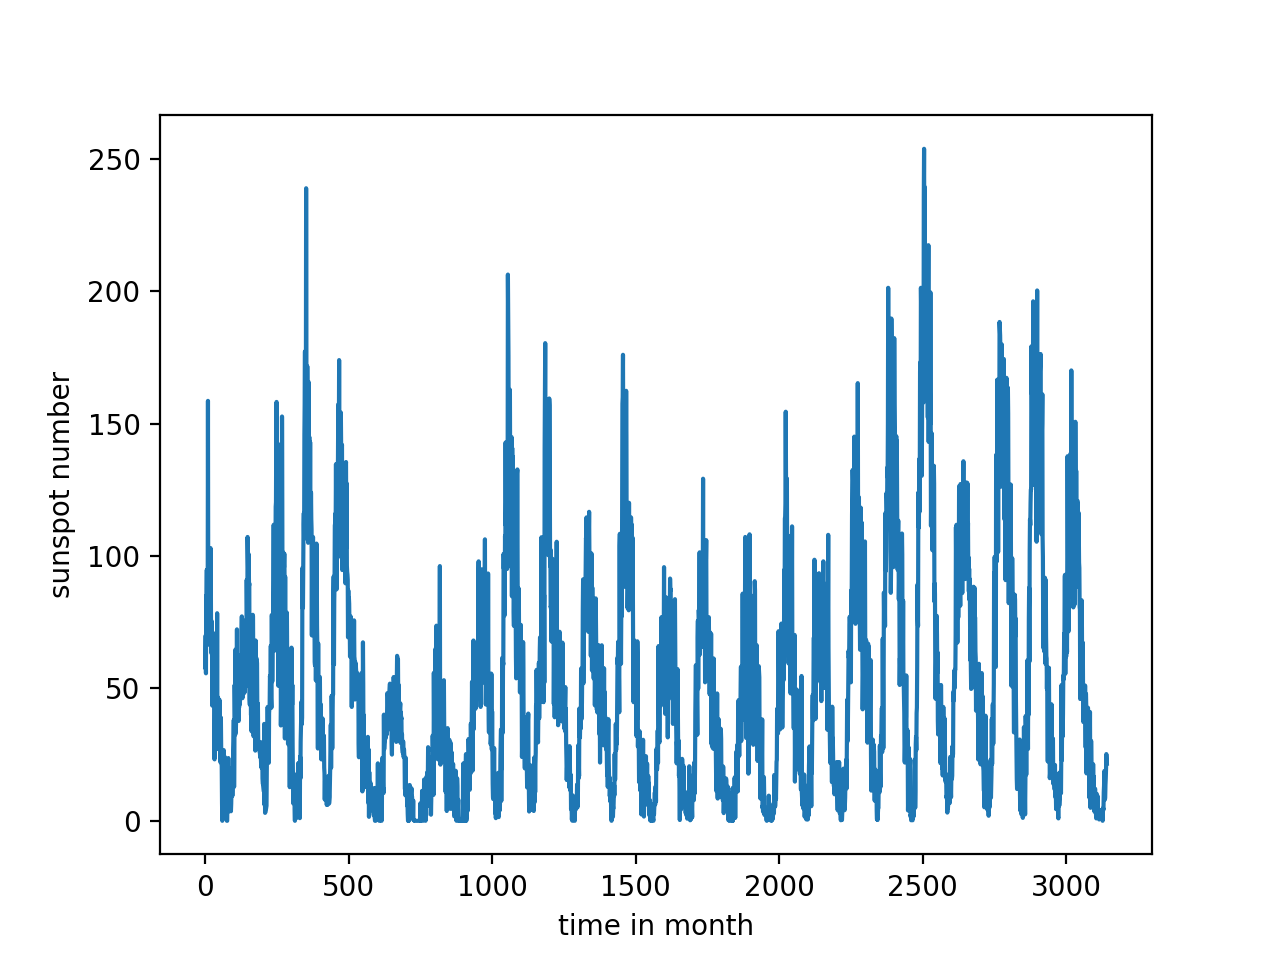
\includegraphics[width=1.\linewidth]{q1a.png}
    \caption{Sunspot Graph as a function of time}
    \end{figure}
    According to different sources (Wikipedia, UCAR, and NASA), the average period of sunspot cycle is around 11-years. That means, in term of months, a period of 132 months. 
    From the graph, we can also estimate the period of solar cycle by counting how many periods it goes through in a fixed period of time. If we zoom into the graph:
    
    \clearpage
    \begin{figure}[h]
    \centering
    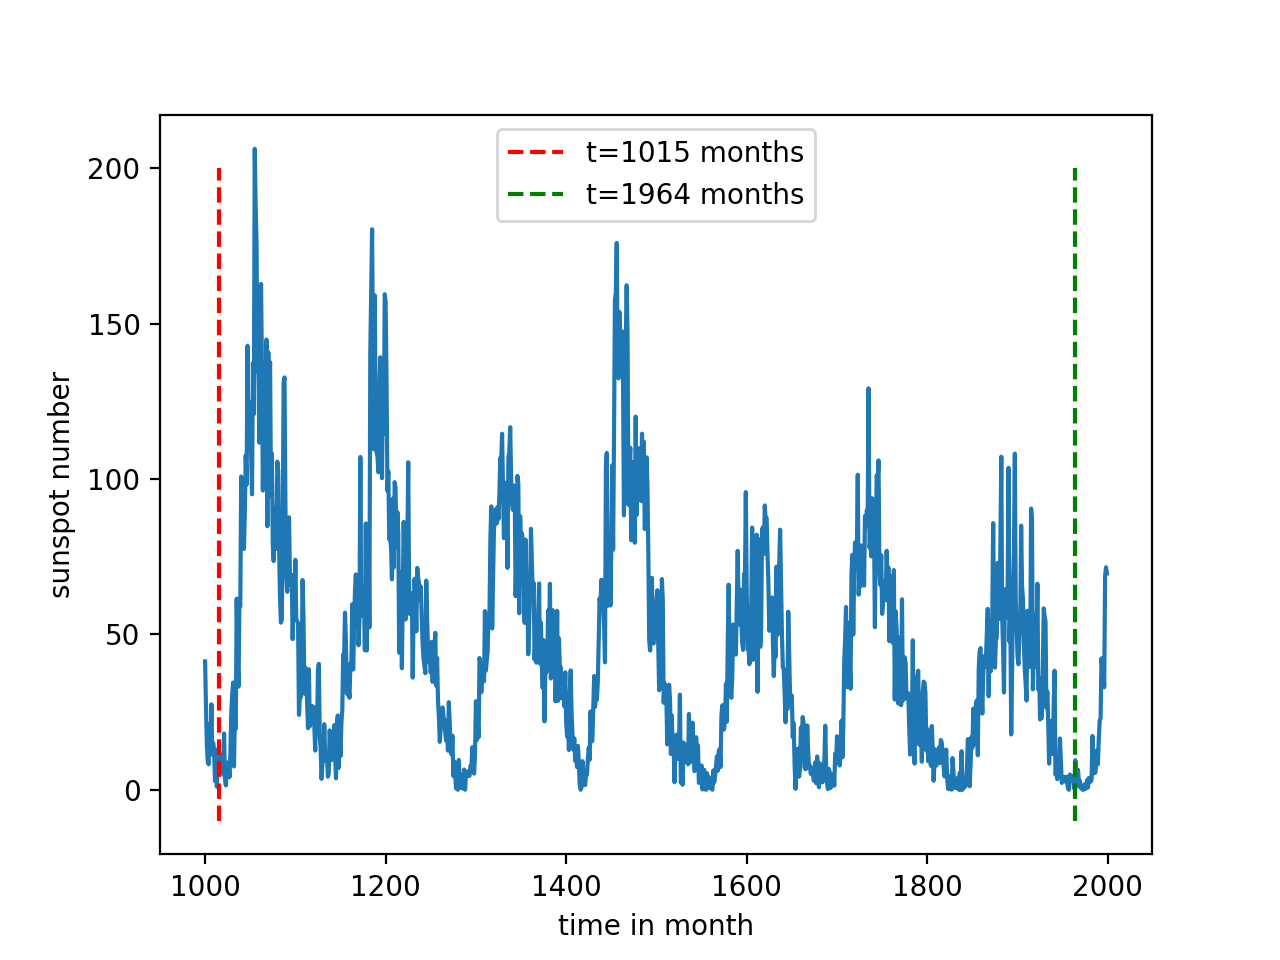
\includegraphics[width=1.\linewidth]{q1b.png}
    \caption{Sunspot Graph as a function of time Zoomed in}
    \end{figure}
    
    It is clearly seen in the graph, that from t=1015 months to t=1964, there are roughly 7 cycles. Calculating the average period,
    \begin{equation}
        \frac{1964  months - 1015  months}{7}=135.57  months
    \end{equation}
    
    So the estimated period is 135.57 months, which is a reasonable estimate comparing to the expected value 132 months.
  \item
    A code for DFT is written according to equation (7.15) from the book, which is:
    \begin{equation}
        c_k=\sum_{n=0}^{N-1}  y_n e^{ -i\frac{2\pi k n }{N}   }
    \end{equation}
    Using the above code, I have constructed the power spectrum of the sunspot data:
    \clearpage

    \begin{figure}[h]
    \centering
    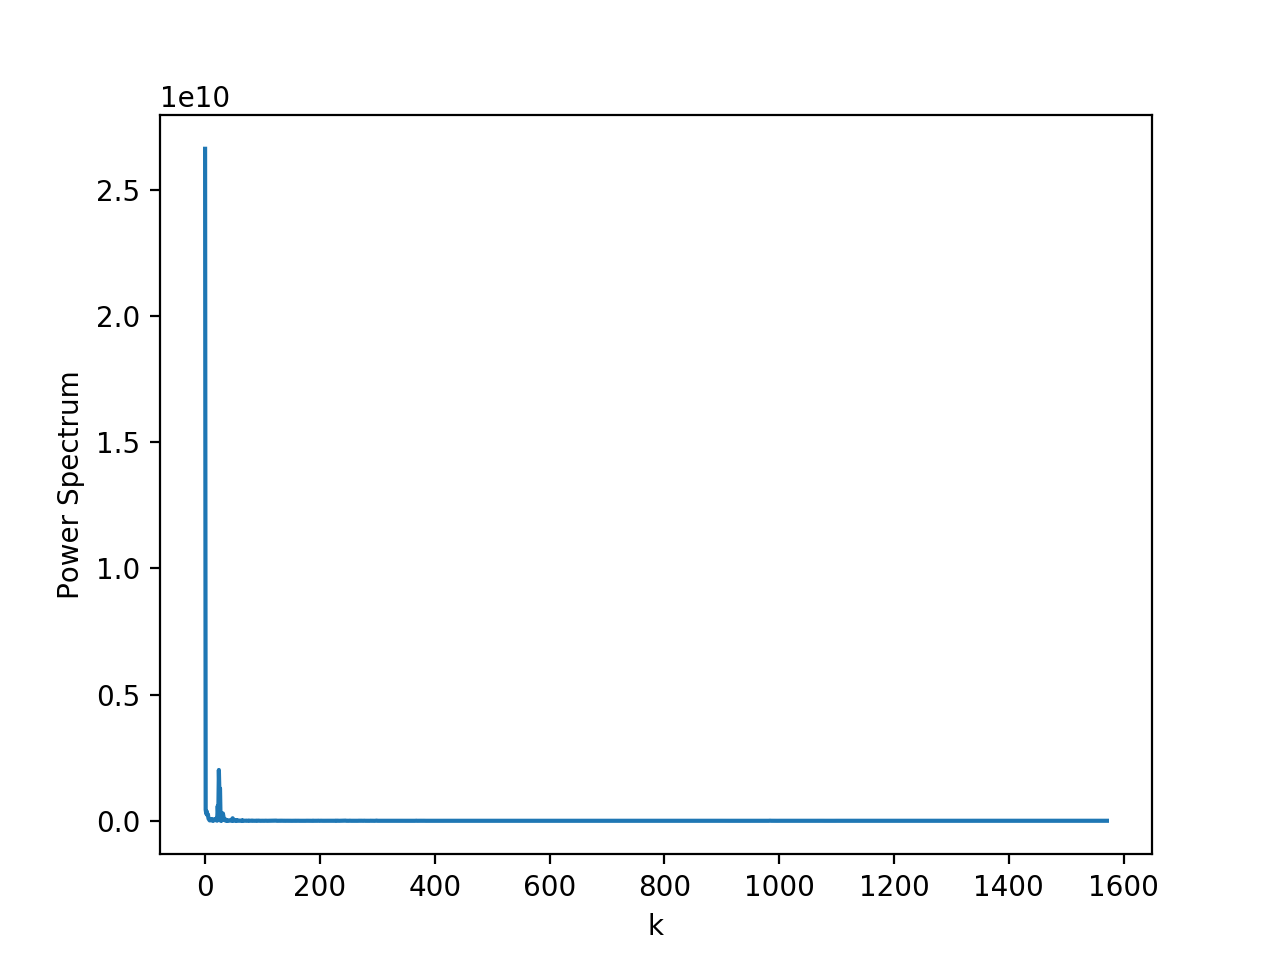
\includegraphics[width=1\linewidth]{q1c.png}
    \caption{The power spectrum of sunspot data}
    \end{figure}
     Figure 3 shows the full power spectrum of the fourier transform. We can clearly see a local maximum around k=20, but to see it clearly we need to zoom in:

    \clearpage
    \begin{figure}[h]
    \centering
    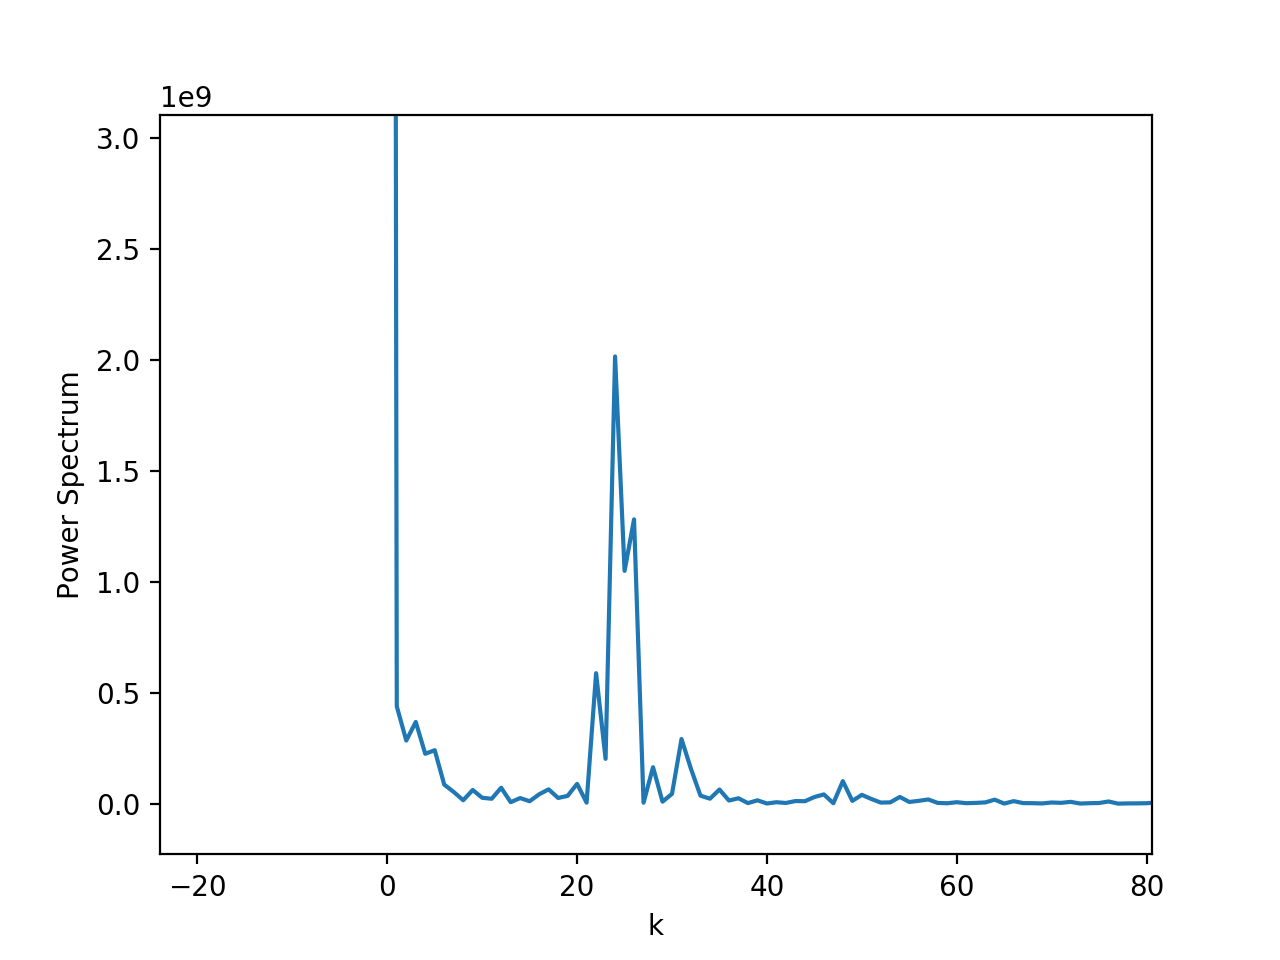
\includegraphics[width=0.8\linewidth]{q1d.png}
    \caption{The power spectrum of sunspot data, zoomed in }
    \end{figure}
    Now we can see that at k=24, there is a local maximum for the power spectrum of the sunspot plot. This is the visible peak that is mentioned in the question.

    \item Transforming from time domain to frequency domain, we use the equation:
    
    \begin{equation}
        f_k=k\frac{f_s}{N}
    \end{equation}
    where $f_k$ is the frequency of the k'th bin in frequency domain, $f_s$ is the sampling rate, and $N$ is the number of points in data. In our case, $f_s$ is once per month. So since we know the dominant frequency is at k=24,
    \begin{equation}
        f_{24}=\frac{24}{3143}month^{-1}=0.0076365month^{-1}
    \end{equation}
    So the period is thus $1/f_{24}$:
    \begin{equation}
        Period=\frac{3143}{24}month=130.958 month
    \end{equation}
    Which is quite close to what I have expected, since the estimated period was 135.57 month. It is certainly very close to the expected value of 132 months period, according to various sources.
    \clearpage
\end{enumerate}


\section*{Problem 2}
\begin{enumerate}
    \item
    I have downloaded the file from the computational physics website, and the picture looks like this:
    \begin{figure}[h]
    \centering
    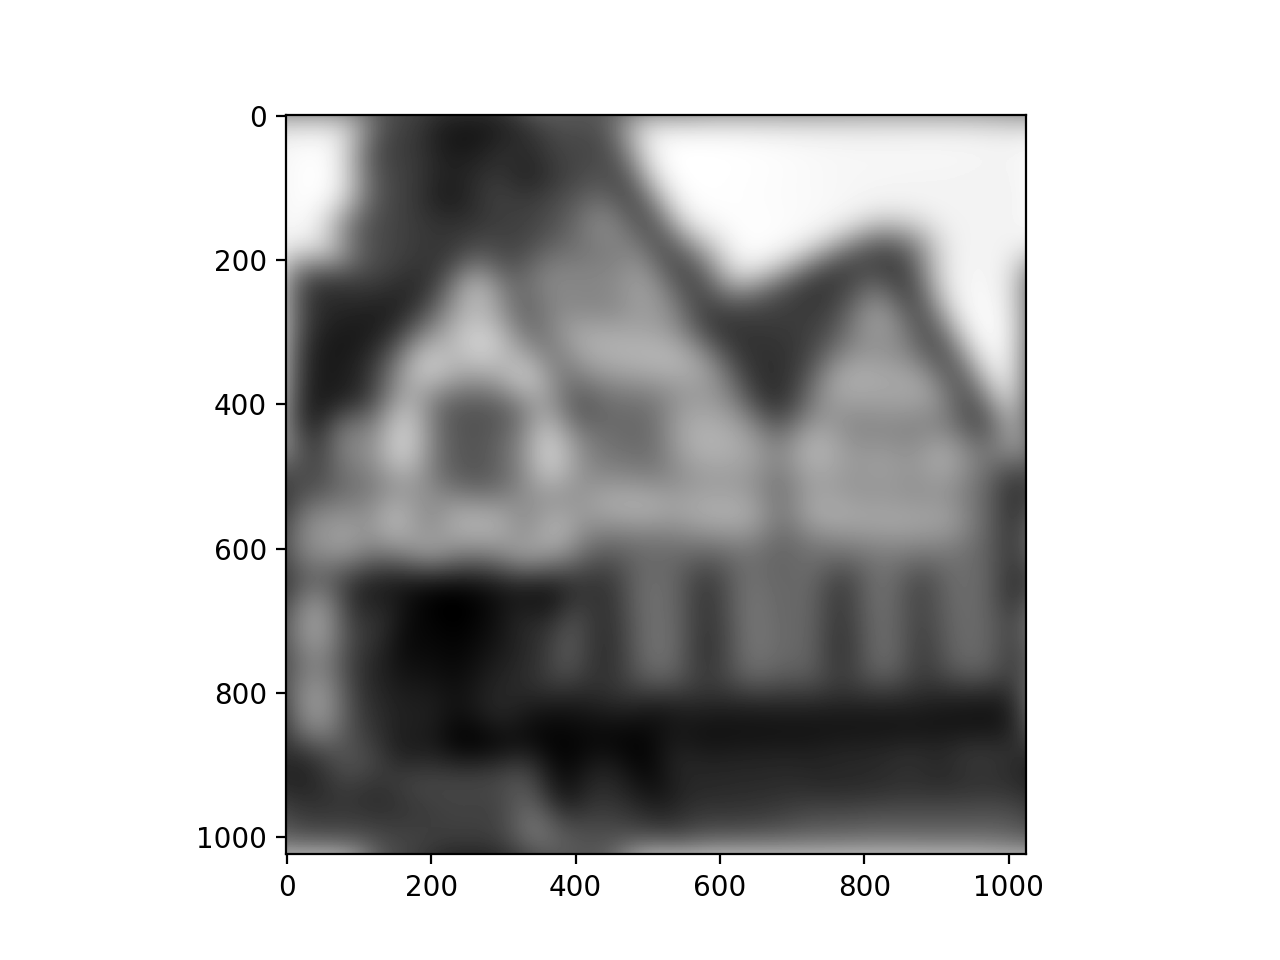
\includegraphics[width=1.\linewidth]{q2a.png}
    \caption{Blurry image}
    \end{figure}
    


    
    \item 
    The Gaussian density plot is constructed using the equaiton:
    \begin{equation}
        f(x,y)=e^{-\frac{x^2+y^2}{2\delta^2}}
    \end{equation}
    
    And since we must apply period boundary condition, I have calculated the density function from (x=0,y=0) to (N/2,M/2), where N and M are the dimension of the image. Then, since we know that the density plot is identical in corners, I can construct the rest of the density plot using it. A picture of the density plot looks like this:
    \begin{figure}[h]
    \centering
    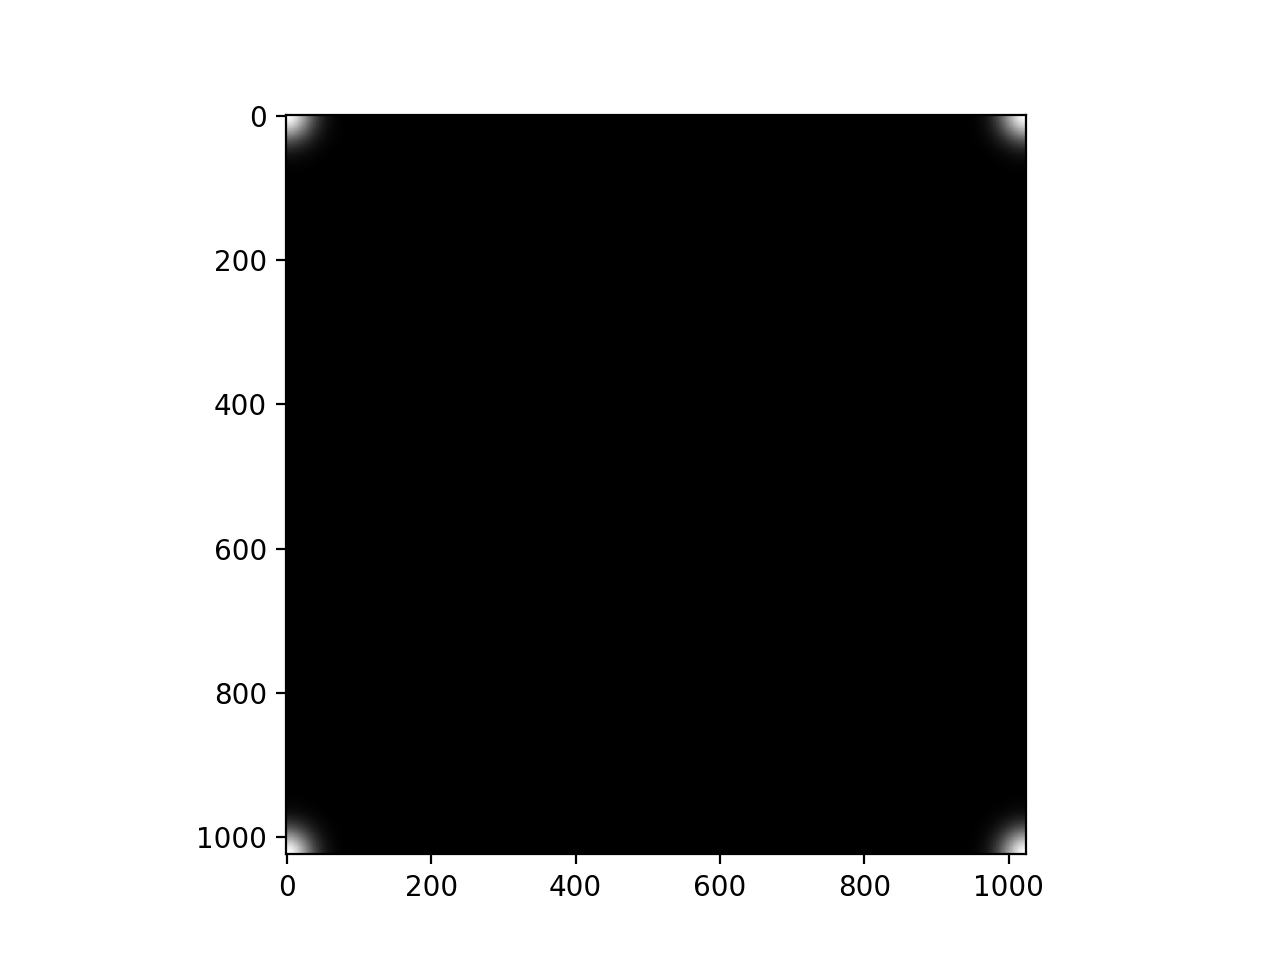
\includegraphics[width=1.\linewidth]{q2b.png}
    \caption{Gaussian density plot with $\delta=25$}
    \end{figure}
    
    

    \item 
    So I first divided the Fourier coefficient of the image by the coefficient of the density plot. Then, where ever the density plot's Fourier coefficient is smaller then $\epsilon$, I change the value back to that of the image's Fourier Transform coefficient. Lastly, I make a inverse Fourier transform of the result, and the deconvoluted image looks like this:
    \clearpage
    \begin{figure}[h]
    \centering
    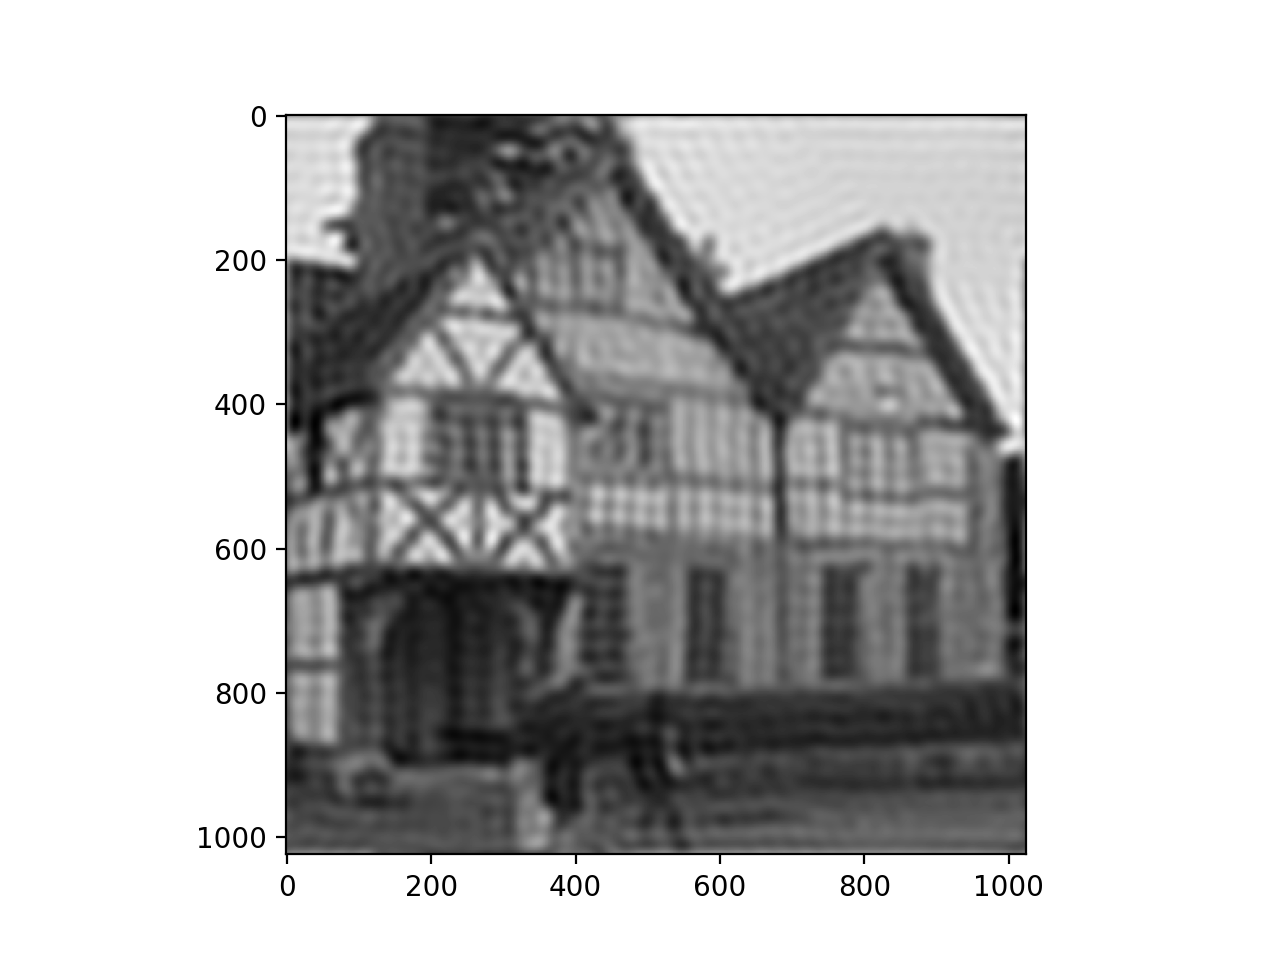
\includegraphics[width=1.\linewidth]{q2c.png}
    \caption{Deconvoluted image}
    \end{figure}
    And the picture definitely looks a lot sharper then it was. It also has weird texture in the image, which I assume is due to the fact that I do not have the exact density plot Fourier transform that was used to calculate the blurred image to begin with. There is bound to be some uncertainty.
    
    \item
    If the image resolution is large, then the Fourier coefficients of the density function will have zeros in them. The math says that, we must divide the zeros to obtain a perfectly accurate original image, and we cannot ignore them like we did for last part. In the mean time, the number of digits that can be stored on computers is limited, so it is unavoidable to have certain error in division involving extremely small number. So, due to the fact that a division involving zero is unavoidable and that I can only store a limited number of digits on my computer, the reconstructed image can never be perfect.
\end{enumerate}
\clearpage
\section*{Reference}
\begin{enumerate}
    \item
    “Solar Cycle.” Wikipedia, Wikimedia Foundation, 6 Oct. 2019
    
    \item
    “The Sunspot Cycle.” The Sunspot Cycle | UCAR Center for Science Education, scied.ucar.edu/sunspot-cycle.
\end{enumerate}

\end{document}
